\subsection{Pianificazione}
    In conformità con la filosofia di sviluppo moderna e dinamica, abbiamo scelto di adottare il modello agile, con un focus specifico sul \textit{framework}\textsubscript{\textit{G}} Scrum.
    Lo Scrum, con le sue pratiche iterative e collaborative, offre una risposta efficace alle sfide e alle mutevoli esigenze del mondo contemporaneo dello sviluppo \textit{software}\textsubscript{\textit{G}}.\\
    Attraverso l'implementazione di Scrum, il nostro team mira a ottenere numerosi benefici positivi che influenzeranno in modo significativo il successo del progetto.
    
\vspace{0.3cm}

\subsubsection*{Vantaggi del Modello Agile e Scrum}
    L'adozione del modello Agile, e in particolare di Scrum, introduce una serie di lati positivi che contribuiranno al raggiungimento dei nostri obiettivi di progetto.
    Alcuni dei principali vantaggi che ci aspettiamo di acquisire includono:

\begin{itemize}
    \item \textbf{Flessibilità e Adattabilità:}
        Lo Scrum consente una rapida risposta ai cambiamenti nei requisiti del cliente, garantendo una maggiore flessibilità durante tutto il ciclo di sviluppo;
    \item \textbf{Collaborazione e Comunicazione:}
        La struttura collaborativa di Scrum promuove una comunicazione aperta e continua tra i membri del team e le parti interessate, migliorando la comprensione reciproca e la condivisione di conoscenze;
        \begin{itemize}
            \item In particolare con l'azienda \textit{proponente}\textsubscript{\textit{G}} sono fissati \textit{SAL}\textsubscript{\textit{G}} \textit{(Stato Avanzamento Lavori)} ogni due settimane.
        \end{itemize}
    \item \textbf{Consegna Incrementale:}
        Attraverso la pratica di rilasci incrementali, Scrum consente la distribuzione graduale delle funzionalità, fornendo valore al cliente fin dalle prime fasi del progetto;
    \item \textbf{Miglioramento Continuo:}
        Le retrospettive regolari incoraggiano il miglioramento continuo del processo, permettendo al team di identificare e risolvere eventuali problematiche in modo tempestivo.
\end{itemize}

La scelta di adottare il modello Agile con Scrum riflette la nostra dedizione a fornire un prodotto di qualità, rispondendo in modo efficiente ai cambiamenti e alle esigenze del cliente.

\subsubsection{Gestione e monitoraggio dell'avanzamento del progetto}
In collaborazione con il \textit{proponente}\textsubscript{\textit{G}}, si è concordato di organizzare l'avanzamento del progetto in periodi di due settimane, seguendo un approccio simile agli sprint della metodologia Scrum. Durante ciascun periodo, in collaborazione con l'azienda e i membri del team, verranno selezionate le \textit{attività}\textsubscript{\textit{G}} da svolgere.

La scelta delle task si baserà sulla loro importanza strategica e sulla fattibilità di completarle entro la durata del periodo. Nel caso in cui alcune \textit{attività}\textsubscript{\textit{G}} non vengano portate a termine entro il periodo determinato, verranno riportate nel consuntivo di periodo e proseguiranno nel periodo successivo.
Ogni periodo sarà documentato attraverso una tabella esaustiva in cui saranno identificate le task relative a ciascun ruolo. Per ogni \textit{attività}\textsubscript{\textit{G}} verrà indicato lo stato di completamento, i tempi previsti ed effettivi, e i costi associati.

%Le \textit{attività}\textsubscript{\textit{G}} assegnate al ruolo "Team" non vengono considerate nel computo dei costi, in quanto sono associate a iniziative di carattere interno e possono essere eseguite da ruoli vari.

%Le ore impiegate per tali \textit{attività}\textsubscript{\textit{G}} sono regolarmente registrate nella sezione "Preventivo orario per membro" presente in ciascun periodo.

Al termine di ciascun periodo, sarà calcolato il costo totale fino a quel momento del progetto, fornendo una chiara visione del progresso complessivo.

Inoltre ogni periodo conterrà una discussione sui rischi occorsi e sull'esito della loro mitigazione seguendo quanto definito in (\ref{sec:AnalisiRischi})

I dati riportati in ciascun periodo rappresentano un riepilogo delle informazioni inserite durante la fase di pianificazione e di preventivazione da parte del responsabile, nonché delle registrazioni orarie effettuate autonomamente dai membri del team tramite il foglio Google condiviso appositamente utilizzato per questo scopo.

\paragraph{Descrizione tabella dei periodi}\label{sec:DescrTabella}\hspace{1pt}

Di seguito è presentata la struttura della tabella che verrà utilizzata per ogni periodo, contenente la pianificazione delle \textit{attività}\textsubscript{\textit{G}}. Nella colonna 'Avanzamento atteso' sono presenti le \textit{attività}\textsubscript{\textit{G}} pianificate suddivise per ruoli e ambiti, indicando il preventivo delle ore e dei costi per ciascuna \textit{attività}\textsubscript{\textit{G}}, oltre al consuntivo che indica se l'\textit{attività}\textsubscript{\textit{G}} è stata completata, con le ore e i costi effettivamente sostenuti.
Ogni \textit{attività}\textsubscript{\textit{G}} contiene le informazioni appena esposte sia per la task, ovvero l'effettivo compito da svolgere,  sia per la verifica che richiede.
La tabella, accessibile a tutto il team come foglio Google condiviso, viene compilata dal responsabile nella sezione relativa alla pianificazione delle \textit{attività}\textsubscript{\textit{G}} e ai preventivi all'inizio del periodo. La parte riguardante il consuntivo viene invece compilata autonomamente dai membri del team.

\vspace{0.5cm}Le \textit{attività}\textsubscript{\textit{G}} elencate nella colonna "Avanzamento atteso" non sono destinate a essere il principale punto di riferimento per i membri riguardo ai compiti da svolgere. Per questo motivo, vengono generate \textit{issue}\textsubscript{\textit{G}} nell'Issue Tracking System (ITS) che sono più esplicative e dettagliate e assegnate ad un unico membro. La colonna "Avanzamento atteso" funge da riferimento generico per le \textit{attività}\textsubscript{\textit{G}} pianificate, permettendo di identificarle per poter allegare i preventivi e i consuntivi associati e comprendere l'incremento apportato da ciascuna di esse.
\begin{figure}[H]
    \centering
    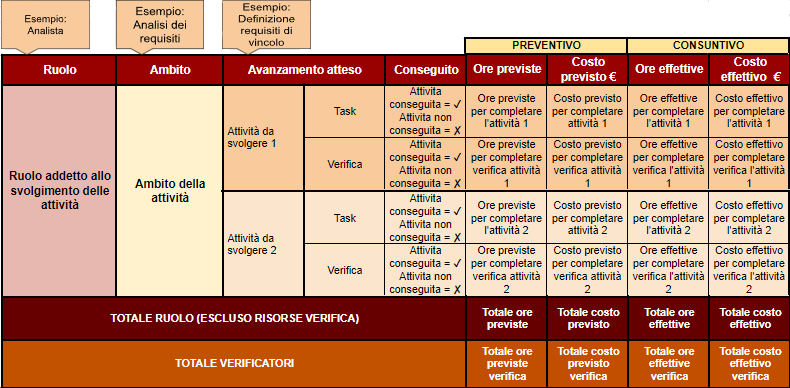
\includegraphics[width=0.9\textwidth]{../Images/spiegazioneTabella.png}
    \caption{Descrizione tabella}
    \label{fig:spiegazioneTabella}
\end{figure}